\documentclass[tikz,border=4pt]{standalone}
\usepackage{tikz}
\usetikzlibrary{arrows.meta, fit, positioning}

\begin{document}
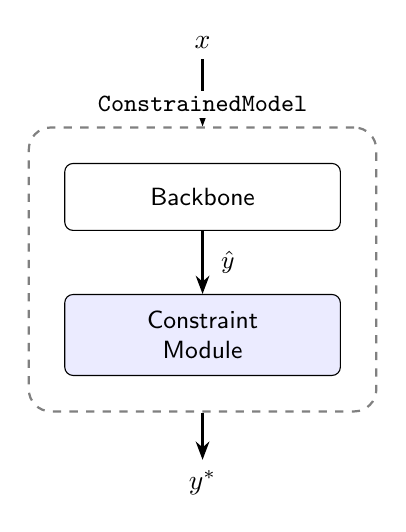
\begin{tikzpicture}[
    font=\sffamily\small,
    >=Stealth,
    block/.style={draw, rounded corners=3pt, fill=white, align=center,
                  inner sep=6pt, minimum width=3.5cm, minimum height=0.85cm},
    cblock/.style={draw, rounded corners=3pt, fill=blue!8, align=center,
                   inner sep=6pt, minimum width=3.5cm, minimum height=0.85cm},
    arrow/.style={->, thick},
]

\node[block] (backbone) at (0, 0) {Backbone};
\node[cblock, below=0.8cm of backbone] (constraint) {Constraint\\Module};

\draw[arrow] (backbone.south)
    -- node[right=3pt, font=\small\sffamily] {$\hat{y}$}
    (constraint.north);

\node[draw, dashed, thick, black!50, rounded corners=8pt, inner sep=0.45cm,
      fit=(backbone)(constraint)] (cm) {};

\draw[arrow] (0, 1.75) node[above, font=\bfseries\sffamily] {$x$} -- (cm.north);

\draw[arrow] (cm.south) -- ++(0,-0.6)
    node[below, font=\bfseries\sffamily] {$y^*$};

\node[above=3pt of cm.north, font=\bfseries\sffamily\small, fill=white, inner sep=2pt]
    {\texttt{ConstrainedModel}};

\end{tikzpicture}
\end{document}
